\documentclass[10pt, oneside,spanish]{article}   	
\usepackage{geometry}
\usepackage{amsmath}
\geometry{a4paper}                   		
\usepackage[utf8]{inputenc}               		
\usepackage{graphicx}												
\usepackage{amssymb}
\usepackage{authblk}
\linespread{1.4}

\title{MKTG 212 - Case 2: Hypothesis Testing and Regression}

\author[]{Juan Manubens}

\affil[]{University of Pennsylvania}
\renewcommand\Authands{, }
\date{}							
\begin{document}
\maketitle

\section{Advertising and Brand Awareness - Long-term Impact}


\begin{itemize}
\item \textbf{[1a] List one advantage and one disadvantage of GMRM splitting up the population into \textit{FWTC} and \textit{FWC} before sampling.}
\end{itemize}

\textbf{\textit{Advantage:}} One advantage of this approach is that it can determine differences in taste for detergents between families with and families without children.

\textbf{\textit{Disadvantage:}} A primary disadvantage of this approach is that it does not necessarily reflect the true proportion of families with/without children in the overall population. By choosing 50 out of each group, it gives the two subpopulations equal weight, but in real life one might be substantially larger (and by extension potentially more lucrative) than the other. 




\begin{itemize}
\item \textbf{[1b] List one advantage and one disadvantage to the way that step (iii) was implemented; that is, by using aided awareness in contrast to unaided awareness.}
\end{itemize}

\textbf{\textit{Advantage:}} An advantage is that the customer will be able to tell you all the brands that he/she knows, even the ones that he/she knows about slightly. Aided awareness mirrors physical retail in that the person will see all the brands before making a purchasing decision, instead of having to think of them independently. 

\textbf{\textit{Disadvantage:}} A disadvantage is that if the consumers need to be prompted to recall a particular brand, the company isn’t sure how memorable their brand name actually is and whether, for example, the customer would be able to look for it in a store or only buy it if he happened to see it on the shelf.

\pagebreak

\begin{itemize}
\item \textbf{[1c] State an appropriate null and alternative hypothesis to test that the awareness BEFORE the advertising was the same in the \textit{FWTC} and \textit{FWC} groups versus the alternative that it was higher in the \textit{FWC} group.}
\end{itemize}
$$ H_0 : p_{FWC} - p_{FWTC} =  0 $$
$$ H_a : p_{FWC} - p_{FWTC} >  0 $$

The null hypothesis states that the difference between the true proportions (of awareness) of the \textit{FWC} and \textit{FWTC} is equal to zero, i.e. they are the same. The alternative hypothesis states that the proportion is higher for the FWC group. 


\begin{itemize}
\item \textbf{[1d] Test the null versus alternative hypothesis from part [1c] at the $\alpha = 0.05$ significance level. Be sure to support your conclusion with the appropriate $t$-statistic and $p$-value.               }
\end{itemize}

$$ p_{FWC} = \frac{18}{50} = 36\%   \quad \textrm{and} \quad   p_{FWTC} =  \frac{12}{50} = 24\% $$
$$ SE[p_{FWC} - p_{FWTC}] = \sqrt[]{\frac{p_{FWC} (1 - p_{FWC})}{n_{FWC}} + \frac{p_{FWTC} (1 - p_{FWTC})}{n_{FWTC}}} $$
$$ \Rightarrow = \sqrt[]{\frac{ 36\%  (1 - 36\% )}{50} + \frac{ 24\%  (1 - 24\% )}{50} } = 9.09\% $$
$$T-statistic = \frac{36\% - 24\%}{9.09\%} = 1.321 < 1.64 = Z_{\alpha=0.05}  $$

We do not reject the null hypothesis since the value of the $t$-test, 1.321, is not significant at the 95\% confidence level (i.e. it does not exceed the $z$-score of 1.64). This means that the proportion of awareness between the two groups is not different at a statistically significant level. 

\begin{itemize}
\item \textbf{[1e] Suppose that you wanted to test the null versus alternative hypothesis that the \textit{overall} fraction of people before the advertising that were aware of CSG was the same as that after the advertising. What additional piece of information would you need to make this assessment?               }
\end{itemize}

We would need to know the proportion of families with and without children in the overall population.  You would multiply the proportion of families with children to the overall population by the proportion with children who had brand recognition and do the same for families without children.









\begin{itemize}
\item \textbf{ [1f]   Test separately at the $\alpha = 0.05$ significance level , for both the \textit{FWTC} and \textit{FWC} groups, that the fraction of people who were aware of CSG BEFORE the advertising is the same as the fraction of people AFTER the advertising, versus the alternative that advertising increased the awareness.  }
\end{itemize}

$$ p_{FWC_{post}} = \frac{28}{50} = 56\%   \quad \textrm{and} \quad   p_{FWC_{prior}} \frac{18}{50} = 36\% $$
$$ SE[p_{FWC_{post}} - p_{FWC_{prior}}] = \sqrt[]{\frac{p_{FWC_{post}} (1 - p_{FWC_{post}})}{n_{FWC}} + \frac{p_{FWC_{prior}} (1 - p_{FWC_{prior}})}{n_{FWC}}} $$
$$ \Rightarrow = \sqrt[]{\frac{ 36\%  (1 - 36\% )}{50} + \frac{ 56\%  (1 - 56\% )}{50} } = 9.77\% $$
$$T-statistic = \frac{56\% - 36\%}{9.77\%} = 2.048 > 1.64 = Z_{\alpha=0.05}  $$

We reject the null hypothesis since the value of the $t$-test, 2.048, is significant at the 95\% confidence level (i.e. it exceeds the $z$-score of 1.64). This means that the proportion of awareness is substantially increased for the group following the advertisements. 


$$ p_{FWTC_{post}} = \frac{14}{50} = 28\%   \quad \textrm{and} \quad   p_{FWTC_{prior}} \frac{12}{50} = 24\% $$
$$ SE[p_{FWTC_{post}} - p_{FWTC_{prior}}] = \sqrt[]{\frac{p_{FWTC_{post}} (1 - p_{FWTC_{post}})}{n_{FWTC}} + \frac{p_{FWTC_{prior}} (1 - p_{FWTC_{prior}})}{n_{FWTC}}} $$
$$ \Rightarrow = \sqrt[]{\frac{ 24\%  (1 - 24\% )}{50} + \frac{ 28\%  (1 - 28\% )}{50} } = 8.76\% $$
$$T-statistic = \frac{28\% - 24\%}{8.76\%} = 0.456 < 1.64 = Z_{\alpha=0.05}  $$

We do not reject the null hypothesis since the value of the $t$-test, 0.456, is not significant at the 95\% confidence level (i.e. it does not exceed the $z$-score of 1.64). This means that the proportion of awareness is not substantially increased for the group following the advertisements. 

\begin{itemize}
\item \textbf{ [1g]  What can you conclude about the long-run effectiveness of advertising?   }
\end{itemize}

The long-run effects of advertising appear to be more substantial for families with children than for families without children. However, we cannot necessarily infer that this association implies causation; for example, there could be another systematic difference between the two groups (that is, a confounding or “lurking” variable) that causes this discrepancy in long-term brand awareness. 




\begin{itemize}
\item \textbf{ [1h]  Do you think that the impact of advertising, as measured here, may be different if an established product (as compared to a new one) was studied? If yes, how? If no, why not?   }
\end{itemize}

Advertising a new product would probably lead a to a higher difference in awareness (since there is no pre-advertising awareness as there would be for an established product). Indeed, if we analyzed the improvement of awareness of a product that was unknown to the customer before the advertising it would be more likely that we found a significant improvement in awareness. This is because standard error would be lower since the left part of the following formula would be zero:

$$ SE[p_{FWTC_{post}} - p_{FWTC_{prior}}] = \sqrt[]{\frac{p_{post} (1 - p_{post})}{n} + \frac{p_{prior} (1 - p_{prior})}{n}} $$

Since the standard error would be lower, the $t$-statistic would be higher. Thus, it would be more likely that it would be higher than the $z$-score. 


\section{Advertising and Brand Awareness - Exposure Effects}


\begin{itemize}
\item \textbf{ [2a]  What proportion of customers saw the advertisement at least once?   }
\end{itemize}

76\% of the customers saw the advertisement at least once (650 out of 850).



\begin{itemize}
\item \textbf{ [2b]  Given that someone is aware of CSG, what is the probability that they did not see the advertisement?   }
\end{itemize}

Given that someone is aware of CSG, there is a 0.18 probability that they did not see the advertisement (80/440). 



\begin{itemize}
\item \textbf{ [2c]   Construct a 99\% confidence interval for the proportion of households that are aware of CSG }
\end{itemize}

99\% confidence interval:
$$ P_{Aware}:\frac{(80+140+220)}{850} = 51.76\% \quad \textrm{with sample size} \quad N = 950 \quad \textrm{and} \quad Z_{\alpha / 2 =0.005} = 2.326 $$

$$ CI: 51.76 \pm 2.326 *  \sqrt[]{\frac{ 51.76 \%  (1 - 51.76 \% )}{950} } = [47.77\% , 55.75\% ] $$


\begin{itemize}
\item \textbf{ [2d]   Test at the $\alpha = 0.01$ significance level that the number of times that a household saw the advertisement is independent of whether or not they are aware of CSG. Provide the relevant $t$-statistic and $p$-value.     }
\end{itemize}

We approached this question by comparing the proportion of people who were aware of the product for people who had seen the advertisement 1-3 and 3+ times against the people who had not seen it respectively. Our results (displayed below) indicate that there is not a significant increase in awareness from watching the advertisement 1-3 times, but that there is a significant increase for those who watched it more than 3 times. 

$$ P_{Aware,x>0}:\frac{80}{200} = 40\% \quad \textrm{v/s} \quad P_{Aware,1\leq x\leq 3}:\frac{140}{290} = 48.27\% \quad \textrm{v/s} \quad P_{Aware,x \geq 3}:\frac{220}{360} = 61.11\% \quad \textrm{v/s} \quad $$


\textbf{"Did not See" (DNS) vs. "Saw 1-3 Times":}

$$ H_0 : P_{Aware,1\leq x\leq 3} - P_{DNS, x=0} =  0 $$
$$ H_a : P_{Aware,1\leq x\leq 3} - P_{DNS, x=0} >  0 $$

$$ SE[P_{Aware,1\leq x\leq 3} - P_{DNS, x=0}] = \sqrt[]{\frac{P_{DNS, x=0} (1 - P_{DNS, x=0})}{n_{DNS, x=0}} + \frac{P_{Aware,1\leq x\leq 3} (1 - P_{Aware,1\leq x\leq 3})}{n_{Aware,1\leq x\leq 3}} } $$
$$ \Rightarrow = \sqrt[]{\frac{ 40\%  (1 - 40\% )}{200} + \frac{ 48.27\%  (1 - 48.27\% )}{290} } = 4.54\% $$
$$T-statistic = \frac{48.27\% - 40\%}{4.54\%} = 1.81 < 2.326  =  Z_{\alpha / 2 =0.005}  $$

We do not reject the null hypothesis since the value of the t-test, 1.81, is not significant at the 99\% confidence level (i.e. it does not exceed the $z$-score of 2.326). This means that there is no statistically significant association between having seen the advertisement 1-3 times and being aware of the product.


\textbf{"Did not See" (DNS) vs. "Saw 3+ Times":}

$$ H_0 : P_{Aware,x \geq 3} - P_{DNS, x=0} =  0 $$
$$ H_a : P_{Aware,x \geq 3} - P_{DNS, x=0} >  0 $$

$$ SE[P_{Aware,x \geq 3} - P_{DNS, x=0}] = \sqrt[]{\frac{P_{DNS, x=0} (1 - P_{DNS, x=0})}{n_{DNS, x=0}} + \frac{P_{Aware,x \geq 3} (1 - P_{Aware,x \geq 3})}{n_{Aware,x \geq 3}} } $$
$$ \Rightarrow = \sqrt[]{\frac{ 40\%  (1 - 40\% )}{200} + \frac{ 61.11\%  (1 - 61.11\% )}{360} } = 4.31\% $$
$$T-statistic = \frac{61.11\% - 40\%}{4.31\%} = 4.89 > 2.326  =  Z_{\alpha / 2 =0.005}  $$

We reject the null hypothesis since the value of the t-test, 4.89, is significant at the 99\% confidence level (i.e. it exceeds the $z$-score of 2.326). This means that  there is a statistically significant (positive, in this case) association between having seen the advertisement more than 3 times and being aware of the product.


\begin{itemize}
\item \textbf{ [2e]   What does your test in (2d) indicate about the long-term effect of advertising, if anything?  }
\end{itemize}

Our answer above shows that significant improvements of long term brand awareness only comes, generally, after the customer sees an advertising several times. In other words, advertising might not produce any noticeable effects in the short-term, but can exhibit benefits in the long term. For this reason, advertising should be part of a long term strategy, and not a tool for immediate benefits. 


\section{Advertising and Brand Awareness - Market Segments} 


\begin{itemize}
\item \textbf{ [3a]  Test at the 95\% confidence level that the mean household income of the \textit{FWTC} Segment is no different than that of the \textit{FWC} Segment versus the alternative that the \textit{FWC} Segment has higher income. Report the $t$-statistic, $p$-value., and conclusion from your test.   }
\end{itemize}

$$ H_0 :  \mu_{FWC} - \mu_{FWTC} =  0 $$
$$ H_a : \mu_{FWC} - \mu_{FWTC} >  0 $$
$$ SE[\mu_{FWC} - \mu_{FWTC}] = \sqrt[]{\frac{SD_{FWTC}^2}{n_{FWTC}} +  \frac{SD_{FWC}^2}{n_{FWC} }} $$
$$ \Rightarrow = \sqrt[]{\frac{ \$10,000^2}{100} + \frac{\$8,100^2 }{100} } = \$1,286.90 $$
$$T-statistic = \frac{\$40,000 - \$36,000}{ \$1,286.90} = 3.11 > 1.64 = Z_{\alpha=0.05}  $$

We reject the null hypothesis that the two groups have the same level of income, since the $t$-test of 3.11 exceeds the one-sided 95\%-confidence $z$-score of 1.64. This means that the \textit{FWC} segment has a higher income than the \textit{FWTC} segment at a statistically significant level.

\begin{itemize}
\item \textbf{ [3b]  Test at the 95\% confidence level that the mean Age of the \textit{FWTC} Segment is no different than that of the \textit{FWC} Segment versus the alternative that the \textit{FWC} segment has lower age.  Report the $t$-statistic, $p$-value., and conclusion from your test.   }
\end{itemize}

$$ H_0 :  \mu_{FWC} - \mu_{FWTC} =  0 $$
$$ H_a : \mu_{FWC} - \mu_{FWTC} <  0 $$
$$ SE[\mu_{FWC} - \mu_{FWTC}] = \sqrt[]{\frac{SD_{FWTC}^2}{n_{FWTC}} +  \frac{SD_{FWC}^2}{n_{FWC} }} $$
$$ \Rightarrow = \sqrt[]{\frac{ 3.5^2}{100} + \frac{3.3^2 }{100} } = 0.481 $$
$$T-statistic = \frac{37-45}{ 0.481} = -16.63 << -1.64 = Z_{\alpha=0.05}  $$

We reject the null hypothesis that the two groups have the same average age, since the value of the t-test of -16.63 is below (i.e. more extreme than) the one-sided 95\%-confidence $z$-score of -1.64. Since the t-test is negative, this means that the \textit{FWC} segment is on average younger than the \textit{FWTC} segment at a statistically significant level.

\begin{itemize}
\item \textbf{ [3c] Explain to someone in words what the difference is between doing a two-sided test versus a one-sided test for parts (3a) and (3b).    }
\end{itemize}

A two-sided test takes into consideration everything that is statistically significantly above or below the desired value, while a one-sided test only counts what is either statistically significantly above or statistically significantly below.  Therefore, you must divide the alpha value by two for two-sided tests, while you don’t for one-sided.  There are some values that pass a one-sided test but not a two-sided one.



\begin{itemize}
\item \textbf{ [3d]   Based on your answers to (3a) and (3b), is the FWC population “preferable” with respect to age and income? State the basis for which you are making that statement, and your conclusion.  }
\end{itemize}

The \textit{FWC} segment appears to be more attractive: it is younger and has a higher level of income, at a statistically significant level. This makes the segment more lucrative from a customer lifetime value perspective, since they will live longer and have more money to spend.

\pagebreak

\section{Hertz Data - Customer Recommendation Predictions} 


\begin{itemize}
\item \textbf{ [4a]  How does recommending Hertz vary with other survey questions, the total cost of the rental \textit{(total-charge-USD)} and the difference (in days) between when people returned the car and when they filled out the survey (\textit{Survey-checkout-diff})? Is there any issue with multicollinearity in your analysis? Please describe your results in decreasing order of the importance of variables.    }
\end{itemize}


\begin{center}
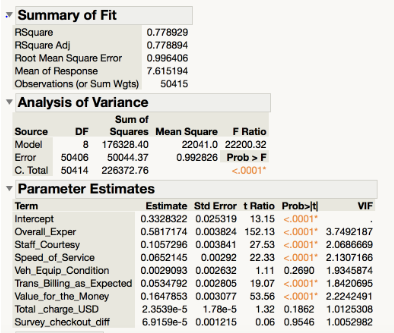
\includegraphics[width=8cm]{4a.PNG}
\end{center}

The survey response for recommending Hertz is dependent on most of the factors we tested; these are ordered and explained below:

\textit{Overall experience} is significant at the 95\%-confidence level. On average, a 1 point increase in overall experience is associated with a 0.58 point increase in recommending Hertz.

\textit{Value for money} is significant at the 95\%-confidence level. On average, a 1 point increase in value for money is associated with a 0.16 point increase in recommending Hertz.

\textit{Staff courtesy} is significant at the 95\%-confidence level. On average, a 1 point increase in staff courtesy is associated with a 0.11 point increase in recommending Hertz.

\textit{Speed of service} is significant at the 95\%-confidence level. On average, a 1 point increase in speed of service is associated with a 0.07 point increase in recommending Hertz.

\textit{Billing as expected} is significant at the 95\%-confidence level. On average, a 1 point increase in billing as expected is associated with a 0.05 point increase in recommending Hertz.

\textit{Vehicle equipment condition, total charge} and \textit{return-difference} in days are not significant at the 95\%-confidence level. 

The intercept is also significant. It implies that if all the associated variables were equal to zero, the expected survey score of recommending Hertz would be 0.33 However, no data reflects this combination of inputs and so it is a rather extreme extrapolation - albeit significant, the value of the integer is virtually meaningless in this case. 

Some of the variables are somewhat collinear: in particular, the overall recommendation score is collinear with the other variables, which makes sense, since we would expect the values of the individual survey questions to influence the overall score. This is reflected by the high variance inflation factor (VIF), which is 3.75. However, none of the VIFs exceed the 5.0 threshold/rule-of-thumb we discussed in class, and are therefore at an acceptable level of collinearity.



\begin{itemize}
\item \textbf{ [4b] Does the above relationship differ based on: }
\end{itemize}

For this question we used JMP to analyze the relationship of recommending Hertz to the same variables than 4(a), but now taking into account whether the location and reason of rental, and the through which the rental was done changed which variables were significantly affected.




\textbf{(1) Where the rental was taken (Airport / Off Airport)?}

As we can see below, the analysis for both Airport and non-airport mirror the results we obtained in 4 (a), thus the location of the airport does not change the affected relationships previously reported:

\begin{center}
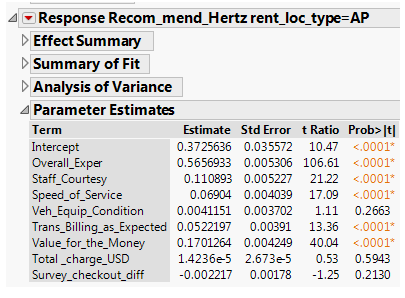
\includegraphics[width=8cm]{4bi.PNG}
\end{center}

\begin{center}
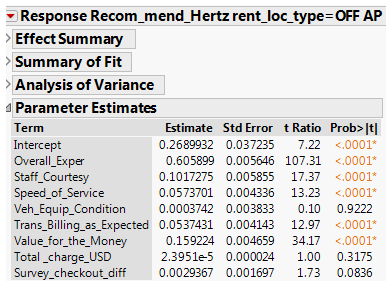
\includegraphics[width=8cm]{4bi2.PNG}
\end{center}

\textbf{(2) Why the rental was taken (Leisure / Business)?}

As we can see below, the analysis for both Leisure and Business mirror the results we obtained in 4 (a), thus the reason of rental does not change the affected relationships previously reported:

\begin{center}
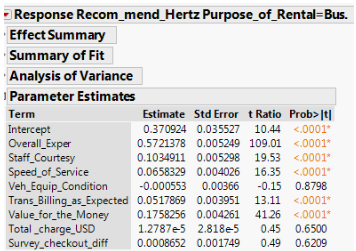
\includegraphics[width=8cm]{4bii.PNG}
\end{center}

\begin{center}
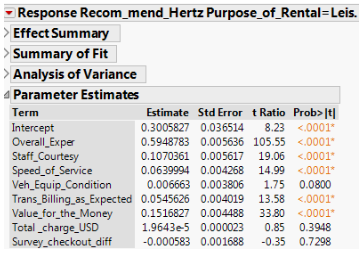
\includegraphics[width=8cm]{4bii2.PNG}
\end{center}

\pagebreak

\textbf{(3) How it was booked i.e., the channel of booking (Booking Channel Dummy)?
}

As we can see below, the analysis for booking through Hertz.com (\textit{Booking-channel-dummy = 1}) does not mirror the previous results and thus channel of booking does have an effect. When booking through Hertz.com the variable \textit{“Veh-Equip-Condition”} also became statistically significant:

\begin{center}
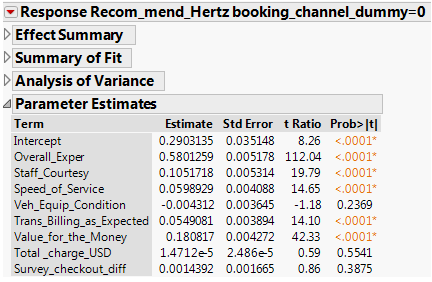
\includegraphics[width=8cm]{4biii.PNG}
\end{center}

\begin{center}
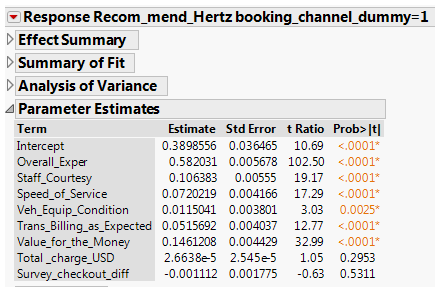
\includegraphics[width=8cm]{4biii2.PNG}
\end{center}
\begin{itemize}
\item \textbf{ [4c]  What other variables will be useful for segmenting customers (beyond the ones I have described above in (b)? Please show the analysis.   }
\end{itemize}

\textbf{Other variables that would be useful in analysis include:}

(1) \textit{Whether the customer got the car type they reserved or not.} To measure this, we ran a simple regression of the recommendation score based on the binary/dummy variable of whether the two variables (reserved type and received type) were equal to each other. We structured it so that people who did not receive the reserved car were coded with a 1, thus expecting a negative coefficient. However, the coefficient was in fact positive and significant: not receiving the car reserved is associated with a 0.07 higher recommendation score. We expect that this is because people generally get a nicer car than the one they requested. Had the data included information about the quality of the different classes we could have tested this hypothesis.

(2) \textit{Canada vs. US address.} We also tested whether survey scores in Canada (or to be precise, from people with addresses in Canada) differed substantially from survey scores of people with US addresses. We also coded this as a dummy variable and set Canadian addresses as 1. We found that there is not a statistically significant difference at the 95\% confidence level, as indicated by the -1.50 $t$-Ratio of the $CN?$-coefficient.

\begin{center}
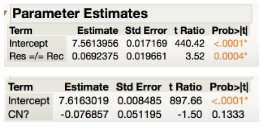
\includegraphics[width=8cm]{4c.PNG}
\end{center}

\begin{itemize}
\item \textbf{ [4d]  What kinds of biases should the Hertz managers be aware of as they evaluate the results from the analysis you have conducted? For each bias, please describe a solution (in words).   }
\end{itemize}

Some of the biases that the Hertz managers should be aware of when evaluating these results include order bias, where the customers’ responses to questions depend on the order in which they were asked.  For example, if a customer who had a favorable experience other than not getting the car he reserved were to be asked only at the very end whether or not he got his reserved car, his answers to the other questions are more likely to be positive because he’d only be prompted to remember the negative experience of not getting the proper car at the very end.  A solution to this bias would be to randomly generate the order of the questions using online software, or to manually place sensitive questions somewhere in the middle in terms of order.  Another bias to watch out for is the leading question bias.  This could occur if Hertz asked, “Hertz is dedicated to providing the highest quality of customer service.  Were you satisfied with your service?”, customers would be encouraged to say yes.  This bias could be eliminated by asking questions without any extra description or qualifiers (simply “Were you satisfied with your service?”). 


\end{document}   
